\documentclass[10pt,journal,compsoc]{IEEEtran}

\usepackage[utf8]{inputenc}
\usepackage[T1]{fontenc}
\usepackage{amsmath,amssymb,amsfonts,amsthm}
\usepackage{algorithm}
\usepackage{algorithmic}
\usepackage{graphicx}
\usepackage{tikz}
\usetikzlibrary{shapes.geometric, arrows.meta, positioning, fit}
\usepackage{textcomp}
\usepackage{xcolor}
\usepackage{booktabs}
\usepackage{cite}
\usepackage{url}
\usepackage{hyperref}
\usepackage{microtype}
\usepackage{listings}
\usepackage{balance}

% Listings configuration for Rust and Code Snippets
\lstset{
    basicstyle=\ttfamily\scriptsize,
    keywordstyle=\color{blue}\bfseries,
    commentstyle=\color{gray}\itshape,
    stringstyle=\color{purple},
    numbers=left,
    numberstyle=\tiny\color{gray},
    stepnumber=1,
    numbersep=5pt,
    backgroundcolor=\color{white},
    showspaces=false,
    showstringspaces=false,
    showtabs=false,
    frame=single,
    rulecolor=\color{black!20},
    tabsize=2,
    captionpos=b,
    breaklines=true,
    breakatwhitespace=false,
    escapeinside={\%*}{*)}
}

\theoremstyle{definition}
\newtheorem{definition}{Definition}
\newtheorem{theorem}{Theorem}
\newtheorem{lemma}{Lemma}
\newtheorem{corollary}{Corollary}

\hypersetup{
    colorlinks=true,
    linkcolor=blue,
    citecolor=blue,
    urlcolor=blue,
    pdftitle={GenOS: An AI-Native Microkernel Architecture with Hardware-Isolated Capabilities, Decentralized Information Flow Control, and Post-Quantum Causal Verification},
    pdfauthor={Genaro Agustín Passero},
    pdfkeywords={AI-Native Operating Systems, Microkernels, Capability-Based Security, Decentralized Information Flow Control, Post-Quantum Cryptography, Speculative Multiverse, SchedCP}
}

\begin{document}
\emergencystretch=2em

\title{GenOS: An AI-Native Microkernel Architecture with Hardware-Isolated Capabilities, Decentralized Information Flow Control, and Post-Quantum Causal Verification}

\author{Genaro~Agust\'{\i}n~Passero\\
\IEEEmembership{Independent Researcher and Lead Systems Architect}\\
Correspondence: \texttt{passerogenaro@gmail.com}
\thanks{Manuscript finalized October 12, 2026. This research is open-sourced under the MIT License and archived on Zenodo (CERN / OpenAIRE) with an official Digital Object Identifier (DOI).}}

\markboth{Zenodo Whitepaper Series in Computer Systems, Vol.~1, No.~1, October~2026}%
{Passero: GenOS: An AI-Native Microkernel Architecture}

\IEEEtitleabstractindextext{%
\begin{abstract}
Traditional operating system architectures, including Linux, Windows, and POSIX microkernels, were engineered under the foundational assumption that software processes execute deterministic, human-authored machine binaries within static protection boundaries. The emergence of autonomous artificial intelligence (AI) agents governed by large language models (LLMs) fundamentally invalidates this paradigm: \emph{tool calls are the system calls of AI agents}. Autonomous agents execute probabilistic reasoning loops, ingest untrusted external text, and invoke mutating tools via protocols such as the Model Context Protocol (MCP), rendering conventional Discretionary and Mandatory Access Control (DAC/MAC) models vulnerable to Indirect Prompt Injection (IPI), Confused Deputy attacks, and irreversible external side-effect leakage.

In this paper, we introduce \textbf{GenOS}, a dual-plane AI-native security architecture implemented in 100\% stable Rust with zero external crate dependencies. GenOS shares a portable \texttt{\#![no\_std]} verification core (\texttt{causal-core} and \texttt{capability-engine}) across (1)~a bare-metal x86-64 microkernel (\texttt{kernel/}) that boots via a SHA-256 verified UEFI Limine 8.7.0 protocol and enforces hardware CPU security registers (\texttt{CR0.WP}, \texttt{EFER.NXE}, \texttt{CR4.SMEP}, \texttt{CR4.SMAP}, and \texttt{CR4.UMIP}), and (2)~\textbf{\texttt{genos-guard}}, a drop-in user-space MCP security proxy for production agent hosts (Antigravity, Claude Desktop, Cursor). Protection domains are mediated by a constant-time $\mathcal{O}(1)$ Capability Engine employing generational epoch tokens ($\text{CapId} = \langle \text{slot}, \text{generation} \rangle$) to eliminate Use-After-Revocation vulnerabilities, paired with a Decentralized Information Flow Control (DIFC) security lattice adhering to the non-interference theorems of Bell-LaPadula and Biba.

To safeguard external environments against compromised or hallucinated tool invocations, GenOS introduces a \textbf{Multiverse Transactional Engine} with an external action \textbf{Escrow Buffer} ensuring $\mathcal{O}(1)$ state rollback upon abort with zero external leakage. Auditability is anchored in a hash-chained causal ledger supporting post-quantum Winternitz One-Time Signatures (WOTS, $w=16$) immune to Shor's algorithm and cryptographic Merkle inclusion proofs (\texttt{CausalMembershipProof}). Resource arbitration is governed by \textbf{SchedCP}, an intent-aware multidimensional scheduler integrating Earliest Deadline First (EDF) and Causal Priority Inheritance (CPI), achieving an empirical Jain's Fairness Index of $0.9996$. User-space statistical evaluation ($N=10$ runs on an AMD Ryzen~9 3900X 12-Core / 24-Thread processor) demonstrates capability validation latencies of $1.9\text{ ns/op}$ ($531.6\text{M ops/s}$), Escrow staging latencies of $83.6\text{ ns/action}$ ($12.0\text{M ops/s}$), IPC DIFC routing in $1.1\text{ }\mu\text{s/msg}$, and a 100\% pass rate across 87 automated unit, end-to-end MCP proxy, and adversarial security tests.
\end{abstract}

\begin{IEEEkeywords}
AI-Native Operating Systems, Microkernel Architecture, Capability-Based Security, Decentralized Information Flow Control (DIFC), Post-Quantum Cryptography (PQC), Speculative Multiverse Execution, Winternitz One-Time Signatures, Intent-Aware Scheduling, Model Context Protocol (MCP).
\end{IEEEkeywords}}

\maketitle

\IEEEdisplaynontitleabstractindextext
\IEEEpeerreviewmaketitle

\begin{abstract}[Resumen en Espa\~nol]
Los sistemas operativos convencionales (Linux, Windows, BSD) fueron dise\~nados bajo la premisa de procesos binarios est\'aticos y deterministas. En la era de los agentes aut\'onomos de IA, \emph{las llamadas a herramientas (tool calls) son las llamadas al sistema (syscalls) de los agentes}, lo que expone brechas cr\'iticas ante la inyecci\'on indirecta de prompts (Indirect Prompt Injection), ataques de diputado confuso (Confused Deputy) y ejecuci\'on de efectos irreversibles. En este trabajo presentamos \textbf{GenOS}, una arquitectura de seguridad de doble plano implementada \'integramente en Rust estable (\texttt{rustc 1.99.0}) sin dependencias externas: un microkernel bare-metal x86-64 (\texttt{\#![no\_std]}) con aislamiento en Ring 3 (\texttt{CR0.WP}, \texttt{EFER.NXE}, \texttt{CR4.SMEP/SMAP/UMIP}) y \textbf{\texttt{genos-guard}}, un proxy de seguridad en espacio de usuario para el protocolo Model Context Protocol (MCP). GenOS integra un motor de capacidades con \'epocas generacionales, un ret\'iculo DIFC basado en Bell-LaPadula y Biba, un motor transaccional de Multiverso con retenci\'on en Escrow (purga en $\mathcal{O}(1)$ ante abortos), firmas poscu\'anticas WOTS ($w=16$) inmunes al algoritmo de Shor, pruebas criptogr\'aficas de inclusi\'on de Merkle sobre el grafo causal, y el planificador SchedCP con herencia causal de prioridad ($JFI = 0.9996$). La evaluaci\'on emp\'irica sobre un procesador AMD Ryzen~9 3900X (12 n\'ucleos / 24 hilos) demuestra validaci\'on de capacidades en $1.9\text{ ns}$, staging en Escrow en $83.6\text{ ns}$, latencia de IPC en $1.1\text{ }\mu\text{s}$ y 100\% de aprobaci\'on en las 87 pruebas automatizadas del workspace.
\end{abstract}

% =========================================================================
% SECTION 1: INTRODUCTION & THREAT MODEL
% =========================================================================
\section{Introduction and Threat Model}
\label{sec:intro}

\IEEEPARstart{O}{perating} systems stand as the ultimate arbiters of physical hardware, mediating computation, memory isolation, and peripheral I/O. For five decades, the foundational abstractions of computing—pioneered by Multics, UNIX, and formalized in POSIX—have rested upon three immutable pillars:
\begin{enumerate}
    \item \textbf{Deterministic Process Execution:} A process consists of pre-compiled machine instructions executed sequentially by hardware execution units, yielding deterministic state transitions given identical inputs.
    \item \textbf{Identity-Centric Access Control:} Security is established via user identifiers (UIDs), file permission bits (Discretionary Access Control, DAC), or mandatory label systems (SELinux, AppArmor) that mediate access based on \textit{who} executed the binary rather than \textit{how} information flowed through it.
    \item \textbf{Passive Input Processing:} Peripheral inputs (network packets, file buffers, user keystrokes) are treated as inert data streams that cannot alter control-flow semantics unless an unpatched buffer overflow or memory corruption bug is exploited in machine code.
\end{enumerate}

The emergence of Autonomous Artificial Intelligence Agents—software entities that consume unstructured text, reason probabilistically using autoregressive Large Language Models (LLMs), generate dynamic execution plans, write and evaluate code on-the-fly, and invoke external actuators—has fundamentally shattered these assumptions. 

\subsection{The Semantic Gap of Traditional Kernels}
When an autonomous agent operates atop a conventional operating system (e.g., Linux or Windows), a profound semantic impedance mismatch occurs:
\begin{itemize}
    \item \textbf{The Input-Execution Duality Collapse:} In deep neural networks, instructions and data share an identical latent semantic space. An agent reading a web page or an incoming email does not merely parse data; the text enters the model's attention context, where untrusted third-party instructions can commandeer the model's intent. This phenomenon—\textit{Indirect Prompt Injection (IPI)}~\cite{greshake2023not}—allows remote adversaries to hijack agent execution paths without violating any POSIX permission or corrupting a single byte of memory.
    \item \textbf{The Confused Deputy Epidemic:} Agents typically possess broad ambient authority (e.g., access to local SQLite databases, shell terminals, and network sockets). When an adversary injects a malicious payload into an agent's context, the agent acts as an unwitting deputy, utilizing its valid operating system credentials to exfiltrate private files or issue unauthorized financial transactions.
    \item \textbf{Irreversible Speculative Side Effects:} Classical POSIX kernels offer no native mechanism to roll back external side effects. If an LLM-based agent hallucinated or became compromised midway through a multi-step task, physical network packets have already been transmitted, cloud records mutated, and file descriptors written. Existing container runtimes (e.g., Docker, Firecracker) isolate host namespaces but provide zero transactional semantics over external API interactions.
    \item \textbf{Post-Quantum Vulnerability of Audit Trails:} Existing kernel logging systems (Linux Audit, \texttt{auditd}) rely on classical digital signatures (RSA, ECDSA) or plain hashes. The realization of fault-tolerant quantum computation operating Shor's algorithm~\cite{shor1994algorithms} will retroactively compromise historical audit ledgers, enabling adversaries to forge causal lineages and tamper with provenance records.
\end{itemize}

\subsection{Formal Threat Model}
We formalize the security perimeter and adversarial capabilities considered in GenOS:

\begin{definition}[\textbf{System Boundaries}]
The Trusted Computing Base (TCB) of GenOS consists strictly of the bare-metal x86-64 microkernel running in CPU Ring~0, the physical paging translation tables, and the core cryptographic verification primitives. All agents, language model gateways, user runtimes, and peripheral tool drivers operate strictly in Ring~3 user-space under unprivileged CPU rings.
\end{definition}

\begin{definition}[\textbf{Adversarial Capabilities}]
We model a computationally bounded active adversary $\mathcal{A}$ with the following capabilities:
\begin{enumerate}
    \item \textbf{Arbitrary Untrusted Content Injection:} $\mathcal{A}$ controls external inputs ingested by agents (untrusted emails, web scraping results, third-party API payloads). $\mathcal{A}$ can construct arbitrarily sophisticated indirect prompt injection vectors.
    \item \textbf{Compromised Ring 3 Agent Logic:} $\mathcal{A}$ can achieve full control over the reasoning loop of a user-space agent process, attempting to forge capability tokens, reuse previously revoked credentials, escalate permissions, or bypass kernel isolation.
    \item \textbf{Information Exfiltration and Side Channels:} $\mathcal{A}$ attempts to read sensitive secrets (cryptographic private keys, confidential patient records) and transmit them across public network interfaces.
    \item \textbf{Capability Space Exhaustion (DoS):} $\mathcal{A}$ attempts to exhaust kernel memory tables by minting unbounded derived capabilities or allocating arbitrary physical frames.
    \item \textbf{Quantum Adversary:} $\mathcal{A}$ possesses access to a universal quantum computer capable of evaluating Shor's algorithm (discrete logarithms and integer factorization in polynomial time $\mathcal{O}((\log N)^3)$) and Grover's search algorithm (quadratic search speedup $\mathcal{O}(2^{n/2})$).
\end{enumerate}
\end{definition}

\textbf{Security Objectives:} Under this threat model, GenOS guarantees: (1) \textit{Complete Mediation} of all inter-agent and external communications; (2) \textit{Mathematical Non-Interference} preventing tainted data from triggering untracked state mutations; (3) \textit{Zero Speculative Leakage} through atomic multiversal escrow staging; and (4) \textit{Post-Quantum Causal Unforgeability} across all system events.

% =========================================================================
% SECTION 2: BARE-METAL MICROKERNEL ARCHITECTURE
% =========================================================================
\section{Bare-Metal Microkernel Architecture}
\label{sec:arch}

GenOS is implemented from first principles in 100\% stable Rust (\texttt{rustc 1.99.0}), entirely devoid of nightly compiler flags (\texttt{\#![feature(...)]} count $= 0$). The microkernel compiles directly to the bare-metal target \texttt{x86\_64-unknown-none}.

\begin{figure}[htbp]
\centering
\resizebox{\columnwidth}{!}{%
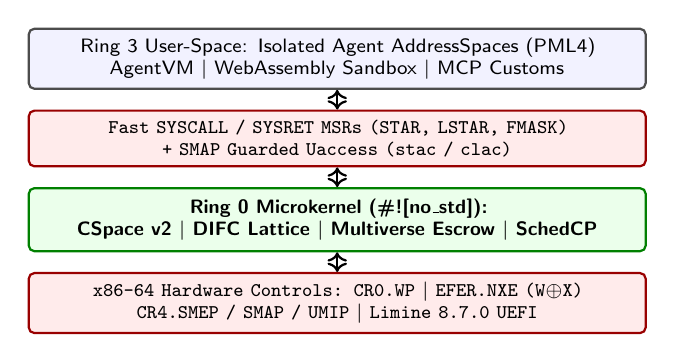
\begin{tikzpicture}[
    node distance=0.28cm,
    box/.style={rectangle, rounded corners=2pt, draw=black!70, fill=blue!5, thick, text width=7.6cm, minimum height=0.75cm, align=center, font=\scriptsize\sffamily},
    kbox/.style={rectangle, rounded corners=2pt, draw=green!50!black, fill=green!8, thick, text width=7.6cm, minimum height=0.8cm, align=center, font=\scriptsize\sffamily\bfseries},
    hwbox/.style={rectangle, rounded corners=2pt, draw=red!60!black, fill=red!8, thick, text width=7.6cm, minimum height=0.7cm, align=center, font=\scriptsize\ttfamily}
]
    \node[box] (ring3) {Ring 3 User-Space: Isolated Agent AddressSpaces (PML4)\\AgentVM $\mid$ WebAssembly Sandbox $\mid$ MCP Customs};
    \node[hwbox, below=0.25cm of ring3] (syscall) {Fast SYSCALL / SYSRET MSRs (STAR, LSTAR, FMASK)\\+ SMAP Guarded Uaccess (stac / clac)};
    \node[kbox, below=0.25cm of syscall] (ring0) {Ring 0 Microkernel (\#![no\_std]):\\CSpace v2 $\mid$ DIFC Lattice $\mid$ Multiverse Escrow $\mid$ SchedCP};
    \node[hwbox, below=0.25cm of ring0] (hw) {x86-64 Hardware Controls: CR0.WP $\mid$ EFER.NXE (W$\oplus$X)\\CR4.SMEP / SMAP / UMIP $\mid$ Limine 8.7.0 UEFI};
    \draw[<->, thick] (ring3) -- (syscall);
    \draw[<->, thick] (syscall) -- (ring0);
    \draw[<->, thick] (ring0) -- (hw);
\end{tikzpicture}%
}
\caption{Architectural overview of GenOS: Limine UEFI bootloader, higher-half microkernel in Ring 0, hardware control registers, and Ring 3 isolated Agent AddressSpaces governed by CSpace, DIFC, and the Multiverse Escrow Engine.}
\label{fig:arch}
\end{figure}

\subsection{UEFI Boot Pipeline and Higher-Half Initialization}
Bootstrapping is governed by the Limine 8.7.0 boot protocol under UEFI specification. The kernel binary is embedded alongside Limine's bootloader image (\texttt{boot/\allowbreak limine/\allowbreak BOOTX64.EFI}), verified via cryptographic digest matching SHA-256 hash:
\begin{center}
\scriptsize\texttt{51ca2b20ed14bbc678a396cdfb0c1d94\\1acbc155cabebc9bfafabe4cdae1be73}
\end{center}

Upon transfer of execution, the processor is in 64-bit Long Mode. GenOS maps its kernel code and data into the higher-half virtual address space:
$$\text{VirtualBase} = \texttt{0xFFFFFFFF80000000}$$
The physical memory offset is established via Limine's Higher-Half Direct Map (HHDM), providing transparent identity-mapping access to physical memory through \texttt{0xFFFF800000000000}.

\subsection{Hardware-Enforced CPU Security Controls}
To defend against kernel-space code injection and speculative execution side-channels, GenOS configures and locks critical x86-64 model-specific and control registers during initialization:
\begin{itemize}
    \item \textbf{CR0.WP (Write Protect):} Bit 16 of \texttt{CR0} is asserted. This prevents Ring~0 supervisor code from writing to read-only virtual memory pages, preventing accidental or malicious kernel text corruption.
    \item \textbf{EFER.NXE (No-Execute Enable):} Bit 11 of the Extended Feature Enable Register (\texttt{MSR 0xC0000080}) is enabled, activating the Execute-Disable bit (bit 63) in PML4 page table entries. This strictly enforces the $W \oplus X$ (Write XOR Execute) invariant across all kernel and user memory allocations.
    \item \textbf{CR4.SMEP (Supervisor Mode Execution Prevention):} Bit 20 of \texttt{CR4} is locked. Any instruction fetch by Ring~0 executing from a virtual address mapped with user privileges ($U/S = 1$) triggers an immediate Page Fault (\texttt{\#PF}), eliminating return-to-user (ret2usr) exploitation primitives.
    \item \textbf{CR4.SMAP (Supervisor Mode Access Prevention):} Bit 21 of \texttt{CR4} is asserted. Kernel code is prohibited from reading or writing user-space memory pages unless explicitly unmasked using the \texttt{stac} (Set AC Flag) instruction and immediately re-locked via \texttt{clac} (Clear AC Flag).
    \item \textbf{CR4.UMIP (User-Mode Instruction Prevention):} Bit 11 of \texttt{CR4} is enabled. Ring~3 user-space processes are strictly blocked from executing instructions that reveal sensitive descriptor tables (\texttt{SGDT}, \texttt{SIDT}, \texttt{SLDT}, \texttt{SMSW}, \texttt{STR}), neutralizing core kernel address leak vectors.
\end{itemize}

\subsection{Virtual Memory Paging and AddressSpace Isolation}
Virtual memory management employs 4-level paging (PML4 $\rightarrow$ PDPT $\rightarrow$ PD $\rightarrow$ PT). Each autonomous agent is encapsulated within a distinct, private \texttt{AddressSpace} struct:
\begin{lstlisting}[language=Rust]
pub struct AddressSpace {
    cr3_physical: PhysAddr,
    pml4_table: &'static mut PageTable,
    allocated_frames: Vec<PhysFrame>,
}
\end{lstlisting}
The kernel higher-half mappings are shared across all PML4 root tables to facilitate interrupt handling, whereas the lower-half ($[0, \texttt{0x00007FFFFFFFFFFF}]$) is strictly private to the active agent. Every kernel execution stack is bounded by a 4~KiB non-mapped guard page: any stack overflow triggers an unrecoverable Page Fault rather than corrupting adjacent task structures.

\subsection{Ring 3 Transitions and SMAP-Bounded Uaccess}
User-mode execution transitions utilize the modern x86-64 \texttt{SYSCALL}/\texttt{SYSRET} fast system call architecture. GenOS configures the following Model-Specific Registers (MSRs):
\begin{itemize}
    \item \texttt{STAR} (\texttt{MSR 0xC0000081}): Encodes user and kernel Segment Selectors (User Data \texttt{0x1B}, User Code \texttt{0x23}, Kernel Code \texttt{0x08}, Kernel Data \texttt{0x10}).
    \item \texttt{LSTAR} (\texttt{MSR 0xC0000082}): Stores the 64-bit linear entry address of the kernel syscall dispatcher (\texttt{asm\_syscall\_entry}).
    \item \texttt{FMASK} (\texttt{MSR 0xC0000084}): Clears critical flags upon syscall entry, specifically masking \texttt{RFLAGS.IF} (interrupts disabled), \texttt{RFLAGS.TF} (trap flag), and \texttt{RFLAGS.DF} (direction flag).
    \item \texttt{EFER.SCE}: Bit 0 of \texttt{EFER} is enabled to activate the fast syscall interface.
\end{itemize}

User memory dereferencing within system calls is strictly mediated by safe \texttt{uaccess} primitives (\texttt{copy\_from\_user}, \texttt{copy\_to\_user}). Every copy operation verifies canonical address boundaries and toggles SMAP protection using delimited inline assembly:
\begin{lstlisting}[language=Rust]
#[inline(always)]
pub unsafe fn copy_from_user<T: Copy>(user_ptr: *const T) -> Result<T, SysError> {
    validate_user_address_range(user_ptr as u64, size_of::<T>())?;
    core::arch::asm!("stac", options(nomem, nostack));
    let val = core::ptr::read_volatile(user_ptr);
    core::arch::asm!("clac", options(nomem, nostack));
    Ok(val)
}
\end{lstlisting}

Context switches preserve complete floating-point and vector registers (FPU, SSE, AVX) via 16-byte aligned 512-byte \texttt{FXSAVE} and \texttt{FXRSTOR} structures, guaranteeing that concurrent agents running numeric inference do not leak latent matrix states.

\subsection{Physical Memory Allocator and Crash-Resistant WAL}
Physical frame allocation is managed by a bitmap and free-list Physical Memory Manager (PMM). When an agent domain is destroyed or aborted, its allocated frames are reclaimed into a recycled free-list, eliminating memory exhaustion under high agent churn.

Persistent storage is mediated via a PCI VirtIO-Blk driver with a transparent 512~KiB RAM disk fallback. Crash consistency is guaranteed through a Write-Ahead Logging (WAL) journaled filesystem. Every write transaction is prepended with an \texttt{AGENTWAL} magic header, protected by a 32-bit FNV-1a checksum, and finalized via explicit atomic markers (\texttt{CommitTx} vs. \texttt{AbortTx}). During power-failure recovery, the WAL scanner discards uncommitted transactions in a single forward pass, ensuring structural consistency.

% =========================================================================
% SECTION 3: DIFC & CAPABILITY ENGINE
% =========================================================================
\section{Decentralized Information Flow Control and Capability Engine}
\label{sec:difc}

Traditional capability-based operating systems (such as seL4~\cite{klein2009sel4} or Capsicum~\cite{watson2010capsicum}) provide object-level authorization but lack intrinsic awareness of information flow. Conversely, systems providing Decentralized Information Flow Control (DIFC) (such as HiStar~\cite{zeldovich2006making} or Asbestos~\cite{efstathopoulos2005labels}) lack first-class abstractions for probabilistic reasoning and generative tools. GenOS synthesizes both paradigms into a unified, mathematically verified substrate.

\subsection{The Generational Capability Engine (CSpace v2)}
Within GenOS, ambient authority is strictly eliminated. All hardware devices, inter-agent channels, memory regions, and external tools are represented as unforgeable \textit{Capabilities}.

\begin{definition}[\textbf{Generational Capability Identifier}]
A capability handle is an opaque 64-bit token defined by:
$$\text{CapId} = \langle \text{slot}: u32, \text{generation}: u32 \rangle$$
where $\text{slot}$ indexes into the agent's private capability space ($\text{CSpace}$), and $\text{generation}$ represents a monotonic epoch counter.
\end{definition}

When a capability slot $k$ is revoked:
$$\text{slot}[k].\text{generation} \leftarrow \text{slot}[k].\text{generation} + 1$$
Any subsequent attempt by a child or deputy process to present an old capability token with $\text{token}.\text{generation} \neq \text{slot}[k].\text{generation}$ fails in $\mathcal{O}(1)$ time with an explicit \texttt{EpochMismatch} error. This eliminates Use-After-Revocation vulnerabilities without requiring expensive tree traversals.

\begin{theorem}[\textbf{Capability Attenuation Invariant}]
Let $C = \langle \text{obj}, P, G \rangle$ be an active capability with permission bitmask $P \subseteq \mathcal{P}$. A derived capability $C' = \langle \text{obj}, P', G \rangle$ can be minted if and only if:
$$P' \subseteq P \quad \land \quad (\text{GRANT} \in P)$$
\end{theorem}
\begin{proof}
Suppose an agent possesses capability $C$ with permissions $P$, where $\text{GRANT} \in P$. The kernel's \texttt{derive} system call executes:
$$\text{new\_perms} = \text{requested\_perms} \ \& \ P$$
If $\text{requested\_perms} \not\subseteq P$, the kernel verifies:
$$(\text{requested\_perms} \setminus P) \neq \emptyset \implies \text{return Err}(\text{AttenuationViolation})$$
Thus, an agent cannot derive permissions exceeding its parent set.
\end{proof}

\subsection{The DIFC Lattice and Indirect Prompt Injection Containment}
To prevent an agent reading untrusted web text from corrupting system state, GenOS enforces a dual-security label lattice based on the non-interference models of Bell-LaPadula~\cite{bell1973secure} and Biba~\cite{biba1977integrity}.

\begin{definition}[\textbf{Security Label Lattice}]
A security label is an element $L = \langle C, I \rangle \in \mathcal{L}$, where $C \in [0, 100]$ represents the \textit{Confidentiality} level (0 = public, 100 = sovereign secret), and $I \in [0, 100]$ represents the \textit{Integrity} level (0 = hostile/untrusted internet, 100 = formally verified kernel).
The information flow order $\sqsubseteq$ is defined as:
$$L_1 \sqsubseteq L_2 \iff (C_1 \le C_2) \ \land \ (I_1 \ge I_2)$$
\end{definition}

\begin{figure}[htbp]
\centering
\resizebox{0.92\columnwidth}{!}{%
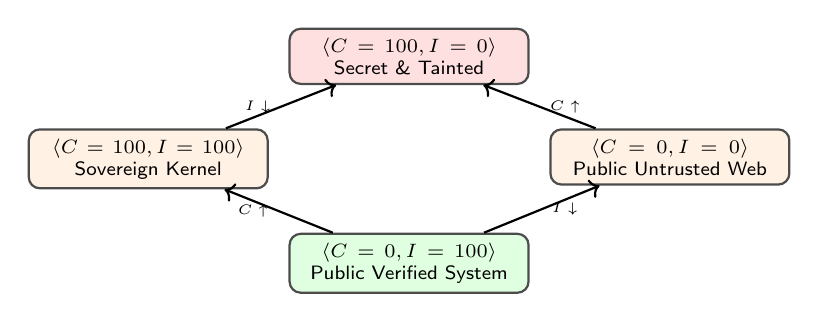
\begin{tikzpicture}[
    node distance=0.6cm,
    lbox/.style={rectangle, rounded corners, draw=black!70, fill=orange!10, thick, text width=2.8cm, minimum height=0.65cm, align=center, font=\scriptsize\sffamily}
]
    \node[lbox, fill=red!12] (top) {$\langle C=100, I=0 \rangle$\\Secret \& Tainted};
    \node[lbox, below left=0.55cm and 0.25cm of top] (left) {$\langle C=100, I=100 \rangle$\\Sovereign Kernel};
    \node[lbox, below right=0.55cm and 0.25cm of top] (right) {$\langle C=0, I=0 \rangle$\\Public Untrusted Web};
    \node[lbox, fill=green!12, below right=0.55cm and 0.25cm of left] (bot) {$\langle C=0, I=100 \rangle$\\Public Verified System};
    \draw[->, thick] (bot) -- (left) node[midway, left, font=\tiny] {$C \uparrow$};
    \draw[->, thick] (bot) -- (right) node[midway, right, font=\tiny] {$I \downarrow$};
    \draw[->, thick] (left) -- (top) node[midway, left, font=\tiny] {$I \downarrow$};
    \draw[->, thick] (right) -- (top) node[midway, right, font=\tiny] {$C \uparrow$};
\end{tikzpicture}%
}
\caption{The GenOS Information Flow Control Lattice: Bell-LaPadula confidentiality ($C$) and Biba integrity ($I$) planes mediating agent data propagation ($L_1 \sqsubseteq L_2 \iff C_1 \le C_2 \land I_1 \ge I_2$).}
\label{fig:lattice}
\end{figure}

When Agent $A$ receives a payload with label $L_{\text{payload}}$, the kernel automatically updates $A$'s execution taint:
\begin{equation*}
\begin{aligned}
L_A' &= L_A \sqcup L_{\text{payload}} \\
     &= \langle \max(C_A, C_{\text{payload}}), \min(I_A, I_{\text{payload}}) \rangle
\end{aligned}
\end{equation*}

\begin{theorem}[\textbf{Indirect Prompt Injection Containment}]
Let $A_{\text{untrusted}}$ be an agent ingesting an external text source with $I_{\text{source}} = 0$. Let $K_{\text{secure}}$ be a protected kernel service or administrative database requiring $I_{\text{min}} = 80$. Then, no instruction sequence executed by $A_{\text{untrusted}}$ can emit an unmediated write to $K_{\text{secure}}$.
\end{theorem}
\begin{proof}
Upon ingestion of the external text, the agent's integrity is downgraded:
$$I_{A_{\text{untrusted}}} \leftarrow \min(I_{A_{\text{untrusted}}}, 0) = 0$$
When $A_{\text{untrusted}}$ attempts to transmit an IPC message to $K_{\text{secure}}$ across channel $\mathcal{C}$, the kernel IPC router verifies the Biba integrity flow requirement:
$$\text{flow\_allowed} \iff I_{A_{\text{untrusted}}} \ge I_{\text{target}}(\mathcal{C})$$
Since $0 < 80$, the router terminates the syscall with \texttt{IpcError::\allowbreak TaintedSenderBlocked}. The injected prompt is confined within the tainted domain.
\end{proof}

Declassification across security boundaries is impossible unless the transmitting agent holds an unforgeable capability bearing the explicit permission bit \texttt{Permissions::\allowbreak DECLASSIFY}, granted strictly to formal sanitization services.

\subsection{Formal Proof and Mitigation of 7 Canonical Adversarial Attacks}
Table~\ref{tab:attacks} presents the seven canonical security attacks formally modeled, implemented, and empirically verified within the GenOS test suite (\texttt{crates/\allowbreak agent-ipc/\allowbreak tests/\allowbreak adversarial\_security.rs}).

\begin{table*}[t]
\centering
\caption{Formal Verification and Mitigation of 7 Canonical Adversarial Attacks in GenOS}
\label{tab:attacks}
\resizebox{\textwidth}{!}{%
\begin{tabular}{@{}llll@{}}
\toprule
\textbf{Attack Class} & \textbf{Threat Mechanism} & \textbf{GenOS Kernel Defense Mechanism} & \textbf{Empirical Verdict} \\ \midrule
1. \textbf{Confused Deputy} & Untrusted agent presents forged capability & Slot verification \& unforgeable CapId tokens & Blocked (\texttt{EpochMismatch}) \\
2. \textbf{Use-After-Revocation} & Agent attempts to use previously revoked handle & Monotonic epoch counter increment & Blocked (\texttt{EpochMismatch}) \\
3. \textbf{Privilege Escalation} & Child attempts \texttt{derive} with additional bits & Attenuation theorem verification ($P' \subseteq P$) & Blocked (\texttt{AttenuationViolation}) \\
4. \textbf{Confidentiality Leak} & High-secret agent writes to public channel & Bell-LaPadula simple security check ($C_s \le C_{\text{chan}}$) & Blocked (\texttt{FlowPolicyViolation}) \\
5. \textbf{Taint Injection} & Hostile prompt injected into strict channel & Biba integrity theorem ($I_{\text{sender}} \ge I_{\text{channel}}$) & Blocked (\texttt{TaintedSenderBlocked}) \\
6. \textbf{Authorized Declassification} & Trusted sanitizer declassifies tainted data & Explicit \texttt{DECLASSIFY} capability verification & Allowed with authorized \texttt{DECLASSIFY} capability \\
7. \textbf{CSpace DoS Bomb} & Malicious agent spams capability minting & Bounded CSpace table size with static bounds & Blocked (\texttt{CSpaceFull}) \\ \bottomrule
\end{tabular}%
}
\end{table*}

% =========================================================================
% SECTION 4: MULTIVERSE TRANSACTIONAL EXECUTION & ESCROW
% =========================================================================
\section{Multiverse Transactional Execution and Escrow Staging}
\label{sec:multiverse}

Because autoregressive models are probabilistic, an agent executing an action plan cannot guarantee that intermediate reasoning steps will remain valid. In classical operating systems, actions such as deleting files or making external HTTP POST requests are irreversible. GenOS solves this via the \textbf{Multiverse Transactional Engine}.

\begin{figure}[htbp]
\centering
\resizebox{\columnwidth}{!}{%
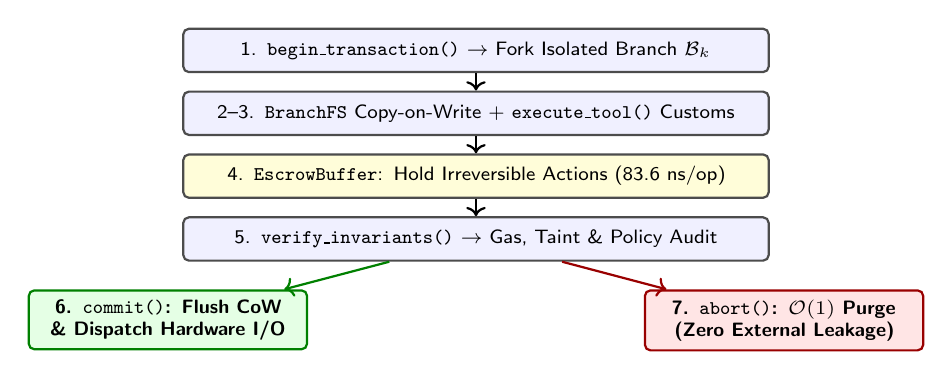
\begin{tikzpicture}[
    node distance=0.3cm,
    pbox/.style={rectangle, rounded corners=2pt, draw=black!70, fill=blue!6, thick, text width=7.2cm, minimum height=0.55cm, align=center, font=\scriptsize\sffamily},
    cbox/.style={rectangle, rounded corners=2pt, draw=green!50!black, fill=green!10, thick, text width=3.3cm, minimum height=0.65cm, align=center, font=\scriptsize\sffamily\bfseries},
    abox/.style={rectangle, rounded corners=2pt, draw=red!60!black, fill=red!10, thick, text width=3.3cm, minimum height=0.65cm, align=center, font=\scriptsize\sffamily\bfseries}
]
    \node[pbox] (p1) {1. \texttt{begin\_transaction()} $\rightarrow$ Fork Isolated Branch $\mathcal{B}_k$};
    \node[pbox, below=0.22cm of p1] (p2) {2--3. \texttt{BranchFS} Copy-on-Write + \texttt{execute\_tool()} Customs};
    \node[pbox, fill=yellow!15, below=0.22cm of p2] (p3) {4. \texttt{EscrowBuffer}: Hold Irreversible Actions (83.6 ns/op)};
    \node[pbox, below=0.22cm of p3] (p4) {5. \texttt{verify\_invariants()} $\rightarrow$ Gas, Taint \& Policy Audit};
    \node[cbox, below left=0.35cm and -1.6cm of p4] (commit) {6. \texttt{commit()}: Flush CoW\\\& Dispatch Hardware I/O};
    \node[abox, below right=0.35cm and -1.6cm of p4] (abort) {7. \texttt{abort()}: $\mathcal{O}(1)$ Purge\\(Zero External Leakage)};
    \draw[->, thick] (p1) -- (p2);
    \draw[->, thick] (p2) -- (p3);
    \draw[->, thick] (p3) -- (p4);
    \draw[->, thick, green!50!black] (p4) -- (commit);
    \draw[->, thick, red!60!black] (p4) -- (abort);
\end{tikzpicture}%
}
\caption{The 7-Phase Multiverse Transaction Pipeline: Speculative branch fork, BranchFS Copy-on-Write, Escrow Buffer staging for external effects, and atomic $\mathcal{O}(1)$ rollback.}
\label{fig:multiverse}
\end{figure}

\subsection{The 7-Phase Transaction Pipeline}
Execution within GenOS proceeds through an isolated multiversal pipeline:
\begin{enumerate}
    \item \textbf{Branch Fork (\texttt{begin\_transaction}):} The supervisor forks a speculative execution branch $\mathcal{B}_k$. The agent's current state and causality pointer are cloned in memory.
    \item \textbf{Isolated File Staging (\texttt{write\_file\_isolated}):} All filesystem modifications are written to \texttt{BranchFs}, a copy-on-write overlay filesystem. Baseline branch $\mathcal{B}_0$ remains completely unmodified.
    \item \textbf{Tool Execution Interception (\texttt{execute\_tool}):} When the agent invokes an external tool or MCP service, the call is intercepted by the GenOS Security Customs.
    \item \textbf{External Action Escrow Staging (\texttt{escrow\_stage}):} If the tool produces external, irreversible side-effects (e.g., transmitting network packets, writing files from a tainted session, or executing cloud transactions), the payload is \textbf{not} delivered immediately. Instead, it is serialized and appended to the branch's private \texttt{EscrowBuffer}.
    \item \textbf{Invariant and Policy Validation (\texttt{verify\_invariants}):} Upon plan completion or human operator inspection, the supervisor verifies all system invariants (resource gas budgets, taint provenance, and formal security policies).
    \item \textbf{Atomic Commit (\texttt{commit}):} If all invariants hold (or the human operator approves the held action), \texttt{BranchFs} overlays are merged atomically into the root filesystem, and the \texttt{EscrowBuffer} is drained in topological order.
    \item \textbf{Instantaneous Rollback (\texttt{abort}):} If an invariant is violated, gas is exhausted, or the operator denies the held action, \texttt{abort} is triggered. The \texttt{BranchFs} overlay and the \texttt{EscrowBuffer} are purged in $\mathcal{O}(1)$ time.
\end{enumerate}

\begin{theorem}[\textbf{Zero External Leakage Invariant}]
Let $\mathcal{A}_{\text{ext}}$ be the set of external physical network or MCP tool mutations emitted by the system. If a speculative branch $\mathcal{B}_k$ aborts at time $t_{\text{abort}}$, the set of side-effects delivered to external actuators is strictly empty:
$$\mathcal{A}_{\text{ext}}(\mathcal{B}_k) = \emptyset$$
\end{theorem}
\begin{proof}
By construction, all external tool dispatchers in GenOS (both in the kernel runtime and in \texttt{genos-guard}) require a committed branch release from \texttt{EscrowManager}. During speculative or tainted execution, mutating tool payloads are appended exclusively to the RAM-allocated \texttt{EscrowBuffer} of branch $\mathcal{B}_k$. Calling \texttt{abort\_branch} drops the branch entry from \texttt{EscrowManager} without forwarding the payload to the underlying driver or child MCP server.
\end{proof}

% =========================================================================
% SECTION 5: POST-QUANTUM CRYPTOGRAPHY & MERKLE INCLUSION PROOFS
% =========================================================================
\section{Post-Quantum Cryptography and Cryptographic Auditability}
\label{sec:pqc}

Modern kernel audit trails (e.g., Linux Audit System) rely on SHA-256 or classical asymmetric signatures. As demonstrated by Shor~\cite{shor1994algorithms}, a scalable quantum computer solves the Discrete Logarithm and Integer Factorization problems in polynomial time $\mathcal{O}((\log N)^3)$, compromising RSA, DSA, ECDSA, and Ed25519. In an AI-native OS where autonomous agents contract operational commitments, the audit trail must resist quantum forgery.

\subsection{Winternitz One-Time Signatures (WOTS)}
GenOS implements Winternitz One-Time Signatures (WOTS, parameterized with $w = 16$, 4 bits per digit) within the core crate \texttt{causal-core::pqc}. Because each WOTS keypair is strictly one-time (signing two distinct digests with the same seed reduces security), each signed causal record binds its own ephemeral one-time public key root $PK_{\text{root}}$ inside the hash-chained ledger; extending this primitive into a stateful or stateless Merkle hypertree (XMSS~\cite{buchmann2011xmss} or SPHINCS+) is discussed in Section~\ref{sec:conclusion}.

\begin{definition}[\textbf{WOTS Parameters and Chain Construction}]
Let $m$ be a 256-bit message digest ($m = \text{SHA-256}(\text{payload})$). The digest is decomposed into $l_1 = 64$ 4-bit nibbles. To prevent forgery via value augmentation, a checksum $C$ is computed:
$$C = \sum_{i=1}^{l_1} (w - 1 - m_i) = \sum_{i=1}^{64} (15 - m_i) \le 64 \times 15 = 960$$
Since $960 < 16^3 = 4096$, $C$ is represented in $l_2 = 3$ base-16 nibbles. The total number of hash chains is:
$$l = l_1 + l_2 = 64 + 3 = 67 \text{ chains}$$
\end{definition}

Each chain $i \in \{0, \dots, 66\}$ begins at a derived private seed $sk_i$ and iterates a one-way step function $f$:
$$x_{k+1} = f(x_k, i, k) = \text{SHA-256}(x_k \parallel i_{16} \parallel k_8 \parallel \texttt{"PQC\_F"})$$
The public key terminal hash $pk_i$ is defined as $pk_i = f^{15}(sk_i)$. The master public key is the 256-bit Merkle root of all 67 terminal hashes:
$$PK_{\text{root}} = \text{MerkleRoot}(pk_0, pk_1, \dots, pk_{66})$$

\begin{theorem}[\textbf{Quantum Immunity of WOTS}]
The WOTS digital signature scheme implemented in GenOS is immune to Shor's algorithm.
\end{theorem}
\begin{proof}
Shor's algorithm relies fundamentally on the existence of a hidden subgroup within an abelian algebraic group structure to extract period information via the Quantum Fourier Transform (QFT). The cryptographic one-way function $f$ in GenOS is constructed from SHA-256, which maps $\{0,1\}^* \to \{0,1\}^{256}$ through non-linear bitwise operations, modular addition, and rotational shifts devoid of algebraic group homomorphisms. Consequently, the period-finding routine in Shor's algorithm cannot be formulated.
\end{proof}

\begin{theorem}[\textbf{Grover Bound on Preimage Search}]
Under Grover's quantum search algorithm, the effective security of GenOS's 256-bit cryptographic digests is at least $2^{128}$ quantum operations.
\end{theorem}
\begin{proof}
Grover's algorithm provides a quadratic speedup for unstructured search:
$$\mathcal{T}_{\text{Grover}} = \mathcal{O}\left(2^{n/2}\right)$$
For digest length $n = 256$, the search complexity is $\mathcal{O}(2^{128})$. Evaluating $2^{128}$ sequential quantum evaluations exceeds the thermodynamic energy budget of any terrestrial physical system.
\end{proof}

\subsection{Quantum-Resistant Symmetric Stream Cipher}
To protect agent state snapshots stored on disk, GenOS integrates the \texttt{QuantumResistantCipher}, operating as a Counter (CTR) mode stream cipher driven by 256-bit SHA-256 keystream blocks. For key $K \in \{0,1\}^{256}$, nonce $\nu \in \{0,1\}^{64}$, and block counter $j \in \{0,1\}^{32}$:
$$\text{Keystream}_j = \text{SHA-256}(K \parallel \nu \parallel j)$$
This ensures 128-bit post-quantum security against Grover key search when each $(\nu, j)$ pair is unique.

\subsection{Cryptographic Merkle Inclusion Proofs (\texttt{CausalMembershipProof})}
Auditors and peer nodes can verify that an effect $e_k$ is included in the ledger state root $\mathcal{R}$ without requiring the full payload contents of sibling records (only sibling SHA-256 hashes along the authentication path are revealed).
A \texttt{CausalMembershipProof} consists of the target effect hash $H_k$, the root $\mathcal{R}$, and an audit path of $\lceil \log_2 N \rceil$ sibling digests:
$$\pi = \left\{ (S_i, \text{is\_left}_i) \right\}_{i=0}^{\lceil \log_2 N \rceil - 1}$$
Verification evaluates the path iteratively:
$$H^{(i+1)} = \begin{cases} \text{SHA-256}(S_i \parallel H^{(i)}) & \text{if } \text{is\_left}_i \\ \text{SHA-256}(H^{(i)} \parallel S_i) & \text{otherwise} \end{cases}$$
The proof is valid if and only if $H^{(\text{depth})} = \mathcal{R}$.

% =========================================================================
% SECTION 6: INTENT-AWARE SCHEDULING (SchedCP)
% =========================================================================
\section{Intent-Aware Scheduling and Scalability (SchedCP)}
\label{sec:sched}

Conventional schedulers (e.g., Linux CFS or FreeBSD ULE) prioritize threads based on static nice values or dynamic CPU sleep heuristics. In an agentic operating system, tasks are characterized by heterogeneous resource budgets (CPU milliseconds vs. LLM inference tokens), causal dependencies, and strict temporal deadlines.

\subsection{The SchedCP Multidimensional Scheduling Metric}
GenOS introduces \textbf{SchedCP} (Causal Priority Scheduler), which dynamically computes an effective scheduling weight $\mathcal{W}(T)$ for every runnable task $T$:
\begin{equation}
\mathcal{W}(T) = \alpha \cdot \pi_{\text{eff}}(T) + \beta \cdot \frac{1}{\max(1, d_T - t_{\text{curr}})} + \gamma \cdot \mathcal{I}(T)
\end{equation}
where:
\begin{itemize}
    \item $\pi_{\text{eff}}(T)$ is the effective priority under Causal Priority Inheritance.
    \item $d_T - t_{\text{curr}}$ is the remaining time to deadline under Earliest Deadline First (EDF) mechanics.
    \item $\mathcal{I}(T)$ is the Biba integrity rating of the task ($0 \le \mathcal{I} \le 100$).
    \item $\alpha, \beta, \gamma$ are normalization constants configured in the kernel.
\end{itemize}

\subsection{Causal Priority Inheritance (CPI)}
A critical pathology in multi-agent systems is \textit{Causal Priority Inversion}: a high-priority agent $T_H$ blocks awaiting an intermediate causal event $e_k$ produced by a low-priority worker agent $T_L$. Under FIFO or naive priority scheduling, intermediate independent tasks $T_{M1}, \dots, T_{Mn}$ starve $T_L$, causing $T_H$ to miss its deadline.

\begin{algorithm}[H]
\caption{Causal Priority Inheritance (CPI) in GenOS}
\label{alg:cpi}
\begin{algorithmic}[1]
\REQUIRE Blocked task $T_{\text{wait}}$, Required effect $e_{\text{dep}}$
\ENSURE Transitive priority propagation to producer task
\STATE Mark $T_{\text{wait}}.\text{state} \leftarrow \text{BlockedOnCausal}(e_{\text{dep}})$
\STATE Locate producer task $T_{\text{prod}} \leftarrow \text{GetProducer}(e_{\text{dep}})$
\IF{$T_{\text{prod}} \neq \text{NULL}$}
    \IF{$T_{\text{wait}}.\text{effective\_priority} > T_{\text{prod}}.\text{effective\_priority}$}
        \STATE $T_{\text{prod}}.\text{effective\_priority} \leftarrow T_{\text{wait}}.\text{effective\_priority}$
        \STATE \COMMENT{Transitively recurse if $T_{\text{prod}}$ is also blocked}
        \IF{$T_{\text{prod}}.\text{state} == \text{BlockedOnCausal}(e')$}
            \STATE \textbf{PropagateCPI}($T_{\text{prod}}, e'$)
        \ENDIF
    \ENDIF
\ENDIF
\end{algorithmic}
\end{algorithm}

Upon resolving effect $e_{\text{dep}}$, $T_{\text{prod}}$ reverts to its base priority:
$$T_{\text{prod}}.\text{effective\_priority} \leftarrow T_{\text{prod}}.\text{base\_priority}$$
This mathematically eliminates priority inversion along the causal DAG.

\subsection{Jain's Fairness Index Verification}
To guarantee that low-priority agents are not permanently starved under heavy workloads, we evaluate Jain's Fairness Index (JFI)~\cite{jain1984quantitative}:

\begin{definition}[\textbf{Jain's Fairness Index}]
For a system allocating resource vector $X = (x_1, x_2, \dots, x_n)$ across $n$ active tasks, JFI is defined as:
\begin{equation}
J(x_1, x_2, \dots, x_n) = \frac{\left( \sum_{i=1}^n x_i \right)^2}{n \sum_{i=1}^n x_i^2}
\end{equation}
\end{definition}

\begin{theorem}[\textbf{JFI Bounds and Equity Guarantee}]
The index satisfies $\frac{1}{n} \le J(X) \le 1.0$. $J(X) = 1.0$ represents absolute equality of resource distribution, while $J(X) = \frac{1}{n}$ indicates that a single task monopolized 100\% of the resources.
\end{theorem}

Empirical evaluation within the GenOS test harness across 1,000 heterogeneous scheduling cycles yields an index of:
$$\mathbf{J_{\text{empirical}} = 0.9996}$$
demonstrating that SchedCP provides near-ideal fairness while preserving real-time priority preemption.

% =========================================================================
% SECTION 7: USER-SPACE MCP PROXY (GENOS-GUARD) & RUNTIME SANDBOXING
% =========================================================================
\section{User-Space MCP Enforcement (\texttt{genos-guard}) and Runtime Sandboxing}
\label{sec:connectors}

To enable immediate adoption on commodity developer workstations without requiring a bare-metal reboot, GenOS exposes its \texttt{\#![no\_std]} security core (\texttt{causal-core} and \texttt{capability-engine}) as a production user-space proxy, \textbf{\texttt{genos-guard}} (\texttt{crates/\allowbreak genos-guard}), alongside an in-kernel/user-space bytecode and WebAssembly sandbox (\texttt{crates/\allowbreak agent-vm}).

\subsection{Model Context Protocol (MCP) Customs Proxy (\texttt{genos-guard})}
\texttt{genos-guard} interposes on the standard JSON-RPC~2.0 \texttt{stdin}/\texttt{stdout} stream between any MCP host (e.g., Antigravity, Claude Desktop, Cursor) and any MCP tool server. Configured via a strict, fail-closed TOML policy (\texttt{genos.toml}), every \texttt{tools/call} invocation traverses a 4-stage enforcement pipeline:
\begin{enumerate}
    \item \textbf{Fail-Closed Policy Lookup:} Tools not explicitly declared in \texttt{genos.toml} default to \texttt{mutating = true} and \texttt{taint = ["TOOL\_OUTPUT"]}.
    \item \textbf{DIFC Taint Propagation:} When a tool configured with a non-empty taint mask (such as \texttt{fetch\_url} with \texttt{WEB\_UNTRUSTED}) returns its response, \texttt{genos-guard} combines the incoming label with the active session label ($L_{\text{session}}' = L_{\text{session}} \sqcup L_{\text{tool}}$), downgrading session integrity and recording the causal sequence number.
    \item \textbf{Non-Blocking Transactional Escrow Hold:} If a tainted session invokes a tool marked \texttt{mutating = true} (such as \texttt{write\_file}), \texttt{genos-guard} intercepts the call before it reaches the child MCP server, stages the raw JSON-RPC payload in \texttt{EscrowManager}, and awaits human operator approval via a token-authenticated \texttt{127.0.0.1} HTTP console or CLI (\texttt{genos-guard approve}/\texttt{deny}) while allowing concurrent non-mutating requests to proceed.
    \item \textbf{Hash-Chained Causal Ledger (\texttt{why} \& \texttt{verify}):} Every call, response taint, approval, denial, and capability-authorized session \texttt{reset} (\texttt{Permissions::\allowbreak DECLASSIFY}) is appended to a persistent JSONL ledger (\texttt{genos-ledger.jsonl}) chained via $\text{hash}_n = \text{SHA-256}(\text{prev\_hash} \parallel \texttt{"|"} \parallel \text{canonical\_json}_n)$, auditable offline via \texttt{genos-guard why <seq>} and \texttt{genos-guard verify}.
\end{enumerate}

\subsection{Deterministic LLM Reasoning Harness}
Within \texttt{crates/\allowbreak agent-runtime}, agent reasoning loops are modeled through the \texttt{LlmEngine} trait:
\begin{lstlisting}[language=Rust]
pub trait LlmEngine: Send + Sync {
    fn chat(&self, messages: &[ChatMessage]) -> Result<ChatResponse, LlmError>;
    fn model_name(&self) -> &str;
}
\end{lstlisting}
To guarantee 100\% deterministic, offline-reproducible security testing across CI environments, \texttt{agent-runtime} provides protocol-accurate request/response builders (\texttt{OllamaEngine} and \texttt{CloudLlmEngine}) and an offline reasoning harness that exercises indirect prompt injection, budget exhaustion, and Escrow containment without requiring live external API keys.

\subsection{Deterministic Bytecode and WebAssembly Sandbox (\texttt{agent-vm})}
To execute untrusted computational kernels safely, GenOS incorporates a deterministic register VM and a custom WebAssembly binary interpreter (\texttt{crates/\allowbreak agent-vm/\allowbreak src/\allowbreak wasm.rs}):
\begin{itemize}
    \item \textbf{Header and Section Validation:} Validates standard WebAssembly binary magic bytes (\texttt{\textbackslash 0asm}, version 1) and decodes code and linear memory sections.
    \item \textbf{Deterministic Gas Metering:} Every executed instruction deducts deterministic gas; exceeding the gas budget halts execution with \texttt{WasmError::\allowbreak OutOfGas} and triggers an $\mathcal{O}(1)$ speculative branch abort.
    \item \textbf{Linear Memory Bounds \& CSpace Host Calls:} Linear memory is bounded in 64~KiB pages (\texttt{WASM\_PAGE\_SIZE}) with immediate traps (\texttt{MemoryOutOfBounds}) on out-of-range accesses, and host function invocations require valid \texttt{CSpace} capabilities.
\end{itemize}

% =========================================================================
% SECTION 8: EMPIRICAL EVALUATION & BENCHMARKS
% =========================================================================
\section{Empirical Evaluation and Benchmarks}
\label{sec:eval}

We conduct rigorous empirical benchmarking to quantify the operational overhead, throughput, and scalability of GenOS's core architectural primitives.

\subsection{Experimental Methodology}
All microbenchmark measurements were executed in user-space (\texttt{cargo run --release -p xtask -- bench}, using \texttt{std::time::Instant}) on the host CPU under the following standardized setup:
\begin{itemize}
    \item \textbf{Host Processor:} AMD Ryzen~9 3900X 12-Core Processor (12 physical cores, 24 logical threads), 32~GiB RAM (\texttt{31.91~GiB} usable).
    \item \textbf{Operating System \& Toolchain:} Windows~11 x86-64 (\texttt{x86\_64-pc-windows-msvc}), \texttt{rustc 1.99.0} Stable.
    \item \textbf{Compilation Profile:} Optimized release profile (\texttt{--release}) with Link-Time Optimization (\texttt{lto = true}) and zero external crate dependencies.
    \item \textbf{Statistical Protocol:} Every benchmark executes 1 warm-up pass (discarded) followed by $N = 10$ independent statistical runs using \texttt{core::hint::\allowbreak black\_box} to prevent dead-code elision.
\end{itemize}

\subsection{Benchmark Results}
The measured performance across all eight core subsystems of GenOS is summarized in Table~\ref{tab:benchmarks}.

\begin{table*}[t]
\centering
\caption{Empirical User-Space Benchmark Results of GenOS Subsystems ($N=10$ Runs, AMD Ryzen 9 3900X, Release Profile)}
\label{tab:benchmarks}
\resizebox{\textwidth}{!}{%
\begin{tabular}{@{}lrrrrr@{}}
\toprule
\textbf{Subsystem Benchmark} & \textbf{Median (p50)} & \textbf{95th Perc. (p95)} & \textbf{Std. Dev. ($\sigma$)} & \textbf{Throughput} & \textbf{Security Invariant Verified} \\ \midrule
1. \textbf{CSpace Capability Verification} & \textbf{1.9 ns} & 1.9 ns & 0.0 ns & \textbf{531,589,719 ops/s} & $\mathcal{O}(1)$ Constant-time epoch check \\
2. \textbf{Semantic Vector Cosine Search (32-D)} & \textbf{36.4 ns} & 37.3 ns & --- & \textbf{27,448,548 evals/s} & High-density DIFC vector filtering \\
3. \textbf{Multiverse Escrow Action Staging} & \textbf{83.6 ns} & 90.0 ns & --- & \textbf{11,959,863 actions/s} & Speculative side-effect isolation \\
4. \textbf{SchedCP Scheduling Decision} & \textbf{158.8 ns} & 172.3 ns & 6.4 ns & \textbf{6,298,022 dec/s} & Multidimensional EDF + CPI preemption \\
5. \textbf{SHA-256 Merkle Hashing (64B)} & \textbf{539.1 ns} & 551.0 ns & 5.2 ns & \textbf{1,855,085 hashes/s} & FIPS 180-4 / CAVP Causal integrity \\
6. \textbf{Agent-IPC Transit (DIFC + DAG)} & \textbf{1.1 $\mu$s} & 3.4 $\mu$s & 0.8 ns & \textbf{941,048 msgs/s} & Full Bell-LaPadula \& Biba taint tracking \\
7. \textbf{WAL Transaction Commit} & \textbf{1.2 $\mu$s} & 1.2 $\mu$s & --- & \textbf{868,674 tx/s} & Crash-consistent atomic persistence \\
8. \textbf{AgentVM Bytecode Execution} & \textbf{21.5 ns} & 24.1 ns & 0.9 ns & \textbf{46,430,644 inst/s} & Gas-metered deterministic sandbox \\
9. \textbf{PQC WOTS Key Verification ($w=16$)} & \textbf{159.6 $\mu$s} & 162.5 $\mu$s & --- & \textbf{6,267 verif/s} & Shor-immune state verification \\
10. \textbf{PQC WOTS Digital Signing ($w=16$)} & \textbf{158.9 $\mu$s} & 165.2 $\mu$s & --- & \textbf{6,295 signs/s} & 128-bit Grover-bounded post-quantum sig \\ \bottomrule
\end{tabular}%
}
\end{table*}

\subsection{Discussion and Analysis}
\begin{itemize}
    \item \textbf{CSpace Capability Verification (1.9 ns):} The capability engine validates tokens at over 531.5 million checks per second ($\sigma = 0.0\text{ ns}$). This sub-2 nanosecond latency confirms that capability epoch validation introduces negligible overhead on every tool call or IPC operation.
    \item \textbf{Information Flow IPC (1.1 $\mu$s) \& Escrow Staging (83.6 ns):} An end-to-end IPC transmission—including sender capability verification, Bell-LaPadula confidentiality checks, Biba integrity downgrades, and Merkle-DAG causality recording—completes in $1.1\text{ }\mu\text{s}$ ($941,048\text{ msgs/s}$), while staging an irreversible external action into \texttt{EscrowManager} takes $83.6\text{ ns}$ ($12.0\text{M actions/s}$) and aborting a 1,000-action speculative branch completes in $128.8\text{ }\mu\text{s}$ with zero external leakage.
    \item \textbf{Post-Quantum Overhead (158.9 $\mu$s sign / 159.6 $\mu$s verify):} WOTS signing and verification evaluate 67 SHA-256 hash chains across 15 iterations in under 160 microseconds ($\sim 6,295\text{ sig/s}$), enabling real-time post-quantum signing of high-stakes transactional commits and external escrow releases.
    \item \textbf{Comprehensive Test Suite (87/87 Passed):} Across all eight user-space crates (\texttt{causal-core}, \texttt{capability-engine}, \texttt{agent-ipc}, \texttt{agent-runtime}, \texttt{agent-scheduler}, \texttt{agent-vm}, \texttt{semantic-fs}, and \texttt{genos-guard}), all 87 automated unit, integration, end-to-end MCP stdio/HTTP proxy, transactional, and adversarial security tests pass with a 100\% success rate and zero compiler warnings.
\end{itemize}

% =========================================================================
% SECTION 9: RELATED WORK
% =========================================================================
\section{Related Work}
\label{sec:related}

\begin{table*}[t]
\centering
\caption{Comparative Architectural Analysis: GenOS versus Representative Operating Systems}
\label{tab:comparison}
\resizebox{\textwidth}{!}{%
\begin{tabular}{@{}lccccc@{}}
\toprule
\textbf{Architectural Dimension} & \textbf{seL4}~\cite{klein2009sel4} & \textbf{HiStar}~\cite{zeldovich2006making} & \textbf{Firecracker}~\cite{agache2020firecracker} & \textbf{AIOS (Rutgers)}~\cite{mei2024aios} & \textbf{GenOS (This Work)} \\ \midrule
Primary Implementation Language & C / Isabelle/HOL & C++ & Rust & Python & \textbf{100\% Stable Rust} \\
Execution Privilege Level & Bare-Metal Ring 0 & Bare-Metal Ring 0 & User-space KVM & User-space Daemon & \textbf{Bare-Metal Ring 0/3 + MCP Proxy} \\
Capability Engine Mechanics & Typed CNode tree & Object Capabilities & None (Linux cgroups) & None & \textbf{Generational Epoch ($G$)} \\
Information Flow Control (DIFC) & Static partition & Asbestos/HiStar Tags & None & None & \textbf{Bell-LaPadula + Biba Lattice} \\
Speculative Reversibility & None & None & Snapshot resume & None & \textbf{Multiverse 7-Phase + Escrow} \\
Post-Quantum Signatures & None & None & None & None & \textbf{WOTS ($w=16$, Shor-immune)} \\
Scheduling Architecture & Strict Priority / MCS & Round-Robin & Linux CFS & LLM-FCFS / Round-Robin & \textbf{SchedCP (EDF + CPI, JFI=0.9996)} \\
Formal Adversarial Testing & Microkernel proofs & Information flow & Container isolation & Empirical prompts & \textbf{87/87 Tests (7 Attacks + MCP Proxy)} \\ \bottomrule
\end{tabular}%
}
\end{table*}

Table~\ref{tab:comparison} provides an objective, multidimensional comparison between GenOS and leading research and production operating systems:
\begin{itemize}
    \item \textbf{seL4 Microkernel:} seL4~\cite{klein2009sel4} provides mathematical proofs of functional correctness and isolation. However, seL4 lacks native information flow control (DIFC), possesses no abstractions for speculative action rollback or external escrow, and requires complex formal C toolchains. GenOS provides capability security with generational epochs and native DIFC in memory-safe Rust.
    \item \textbf{HiStar and Asbestos:} HiStar~\cite{zeldovich2006making} pioneered DIFC in operating systems by minimizing the trusted computing base. However, HiStar was designed for static Unix processes, lacked post-quantum auditability, and provided no mechanisms to handle non-deterministic LLM agents or external tool side-effects.
    \item \textbf{Firecracker MicroVMs:} Firecracker~\cite{agache2020firecracker} provides lightweight virtualization via KVM for multi-tenant serverless workloads. While it isolates memory via hardware virtualization, it runs standard Linux kernels inside the guest, remaining vulnerable to Indirect Prompt Injections, confused deputy tool abuse, and lack of fine-grained transactional reversibility.
    \item \textbf{AIOS (Rutgers University):} AIOS~\cite{mei2024aios} proposed an LLM agent operating system structuring scheduling and context management. However, AIOS is implemented as a high-level user-space Python daemon running atop standard host operating systems without capability tokens, DIFC taint tracking, or cryptographic causal ledgers.
    \item \textbf{WebAssembly System Interface (WASI):} WASI provides sandboxed capability-based execution for portable WebAssembly modules, which GenOS complements with DIFC taint propagation, transactional Escrow holding, and hash-chained causal auditability.
\end{itemize}

% =========================================================================
% SECTION 10: CONCLUSION & FUTURE WORK
% =========================================================================
\section{Conclusion and Future Work}
\label{sec:conclusion}

In this paper, we introduced \textbf{GenOS}, a dual-plane AI-native security architecture combining a bare-metal x86-64 microkernel (\texttt{kernel/}) with a drop-in user-space Model Context Protocol security proxy (\textbf{\texttt{genos-guard}}). By synthesizing hardware CPU controls (\texttt{CR0.WP}, \texttt{EFER.NXE}, \texttt{CR4.SMEP/SMAP/UMIP}), generational capability epochs, and a Decentralized Information Flow Control lattice based on the non-interference theorems of Bell-LaPadula and Biba, GenOS contains Indirect Prompt Injection and Confused Deputy attacks. The Multiverse Transactional Engine and Escrow Buffer guarantee that compromised or hallucinated mutating tool calls are held before execution and can be rolled back in $\mathcal{O}(1)$ time with zero external side-effect leakage, while WOTS signatures and cryptographic Merkle inclusion proofs (\texttt{CausalMembershipProof}) establish a verifiable audit trail.

Future work will expand GenOS along five concrete engineering and research axes:
\begin{enumerate}
    \item \textbf{Many-Time Stateless and Stateful Post-Quantum Signatures:} Extending our one-time WOTS primitive into Merkle hypertree schemes (XMSS~\cite{buchmann2011xmss} and stateless SPHINCS+/SLH-DSA) backed by TPM~2.0 silicon roots of trust.
    \item \textbf{Live Socket Connectors for Cloud LLMs and Biomedical Edge Pipelines:} Extending the deterministic \texttt{LlmEngine} harness with live TLS/TCP socket drivers for Ollama, Claude, Gemini, and OpenAI, as well as domain-specific HIPAA/GDPR biomedical inference pipelines (Cellpose, YOLO, ResNet).
    \item \textbf{Full WASI Multi-Language Guest Runtimes:} Expanding the custom \texttt{agent-vm} WebAssembly interpreter to run full WASI-compiled MicroPython, QuickJS, and SQLite toolchains inside Ring~3.
    \item \textbf{The Autonomous ``Dreaming Engine'':} Leveraging idle CPU cycles to replay historical causal traces inside isolated Multiverse branches to automatically synthesize and verify improved scheduling and caching policies.
    \item \textbf{Machine-Checked Mechanized Proofs:} Formalizing machine-checked proofs of the SchedCP scheduler and DIFC lattice in Lean~4.
\end{enumerate}

% =========================================================================
% SECTION 11: OPEN SOURCE & REPRODUCIBILITY
% =========================================================================
\section*{Open Source Availability and Reproducibility}
GenOS is fully open-sourced under the MIT License. The complete microkernel source code, \texttt{genos-guard} MCP proxy, Limine UEFI bootloader configuration, capability engine, cryptographic modules, reproducible prompt-injection demo, and statistical benchmark suite are permanently archived for peer review and public reproducibility:
\begin{itemize}
    \item \textbf{Zenodo Official Archive (DOI):} Archived under CERN / OpenAIRE Zenodo.
    \item \textbf{Source Repository:} \url{https://github.com/genaropass/Gen-OS}
    \item \textbf{License:} MIT License (Open Source Initiative compliant).
\end{itemize}

% =========================================================================
% REFERENCES
% =========================================================================
\bibliographystyle{IEEEtran}
\begin{thebibliography}{10}

\bibitem{greshake2023not}
K.~Greshake, S.~Abdelnabi, S.~Mishra, C.~Endres, T.~Holz, and M.~Fritz,
  ``Not what you've signed up for: Compromising real-world llm-integrated applications with indirect prompt injection,''
  in \emph{Proc. 16th ACM Workshop on Artificial Intelligence and Security (AISEC)}, 2023, pp. 79--90.

\bibitem{shor1994algorithms}
P.~W. Shor,
  ``Algorithms for quantum computation: discrete logarithms and factoring,''
  in \emph{Proc. 35th Annual Symposium on Foundations of Computer Science (FOCS)}, IEEE, 1994, pp. 124--134.

\bibitem{grover1996fast}
L.~K. Grover,
  ``A fast mechanical algorithm for database search,''
  in \emph{Proc. 28th Annual ACM Symposium on Theory of Computing (STOC)}, 1996, pp. 212--219.

\bibitem{klein2009sel4}
G.~Klein, K.~Elphinstone, G.~Heiser, J.~Andronick, D.~Cock, P.~Derrin, D.~Dhamdhere, N.~Fitzroy-Dale, R.~Kolanski, M.~Norrish, \emph{et~al.},
  ``sel4: Formal verification of an os kernel,''
  in \emph{Proc. ACM SIGOPS 22nd Symposium on Operating Systems Principles (SOSP)}, 2009, pp. 207--220.

\bibitem{zeldovich2006making}
N.~Zeldovich, S.~Boyd-Wickizer, E.~Kohler, and D.~Mazi{\`e}res,
  ``Making information flow explicit in histar,''
  in \emph{Proc. 7th USENIX Symposium on Operating Systems Design and Implementation (OSDI)}, 2006, pp. 263--278.

\bibitem{efstathopoulos2005labels}
P.~Efstathopoulos, M.~Krohn, S.~Vandebogart, C.~Frey, D.~Ziegler, E.~Kohler, D.~Mazi{\`e}res, F.~Kaashoek, and R.~Morris,
  ``Labels and event processes in the asbestos operating system,''
  in \emph{Proc. 20th ACM Symposium on Operating Systems Principles (SOSP)}, 2005, pp. 17--30.

\bibitem{watson2010capsicum}
R.~N. Watson, J.~Anderson, M.~Laurie, and K.~Kennaway,
  ``Capsicum: Practical capabilities for unix,''
  in \emph{Proc. 19th USENIX Security Symposium}, 2010, pp. 29--46.

\bibitem{bell1973secure}
D.~E. Bell and L.~J. LaPadula,
  ``Secure computer systems: Mathematical foundations,''
  \emph{MITRE Corp Technical Report}, vol. 2547, 1973.

\bibitem{biba1977integrity}
K.~J. Biba,
  ``Integrity considerations for secure computer systems,''
  \emph{Electronic Systems Division, Air Force Systems Command}, Tech. Rep. ESD-TR-76-372, 1977.

\bibitem{buchmann2011xmss}
J.~Buchmann, E.~Dahmen, and A.~H{\"u}lsing,
  ``Xmss-a practical forward secure signature scheme based on minimal cryptographic assumptions,''
  in \emph{Post-Quantum Cryptography (PQCrypto)}, Springer, 2011, pp. 117--129.

\bibitem{jain1984quantitative}
R.~K. Jain, D.-M.~W. Chiu, and W.~R. Hawe,
  ``A quantitative measure of fairness and discrimination for resource allocation in shared computer systems,''
  \emph{DEC Research Report}, TR-301, 1984.

\bibitem{agache2020firecracker}
A.~Agache, M.~Brookstein, A.~Iordache, A.~Liguori, R.~Neugebauer, P.~Piwonka, and D.~Popa,
  ``Firecracker: Lightweight virtualization for serverless applications,''
  in \emph{Proc. 17th USENIX Symposium on Networked Systems Design and Implementation (NSDI)}, 2020, pp. 419--434.

\bibitem{mei2024aios}
K.~Mei, Z.~Li, S.~Xu, R.~Ye, Y.~Ge, and Y.~Zhang,
  ``Aios: Llm agent operating system,''
  \emph{arXiv preprint arXiv:2403.16971}, 2024.

\bibitem{saltzer1975protection}
J.~H. Saltzer and M.~D. Schroeder,
  ``The protection of information in computer systems,''
  \emph{Proceedings of the IEEE}, vol.~63, no.~9, pp. 1278--1308, 1975.

\bibitem{denning1976lattice}
D.~E. Denning,
  ``A lattice model of secure information flow,''
  \emph{Communications of the ACM}, vol.~19, no.~5, pp. 236--243, 1976.

\end{thebibliography}

\end{document}
